\newpage
\section{Implementation}
	\subsection{Video Controller}
        \subsubsection{VGA Controller}
        \subsubsection{HDMI Controller}
    \subsection{Image Generator}
	\begin{figure}[here]
		\centering
		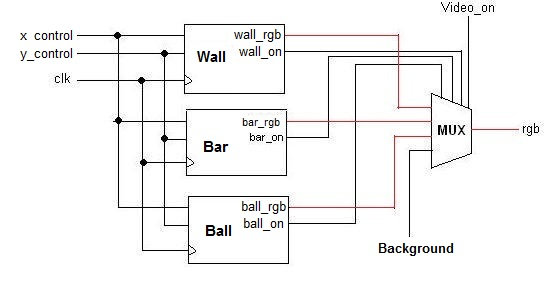
\includegraphics[scale=0.7]{images/img_gen.jpg}
		\caption{Schematic of the Image Generator}
		\label{img_gen}
	\end{figure}
        The Image Generator takes inputs from the players and outputs the video that can be displayed through the HDMI interface of the Atlys board. The panels shown in figure \ref{ball_wall_panel} are submodules of the module \texttt{image\_generator\_c}.
		This module calculates the movement of the ball and movement the two panels that are controlled by the players. 
		
		The movement of the ball is done by the \texttt{ball\_c} module. (see next Section for more details on implementation).
		After a well determined time frame, the ball's movement direction is determined and the next \texttt{x\_pos} and \texttt{y\_pos} are either incremented or decremented. 
		
		The module \texttt{panel\_c} determines the y-coordinate of on panel based on the player input. For instance, pressing \texttt{btn\_up} increments the \texttt{y\_pos} signal if the panel did not reach the top edge already. 


    \subsection{Match Controller}
    \subsection{Sound Generator}
        In order to generate sound, we used the on board LM4550 chip
	\begin{figure}[here]
		\centering
		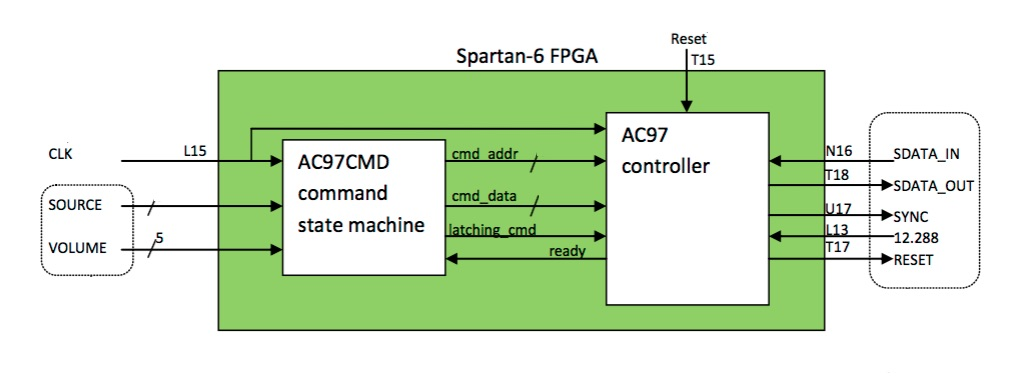
\includegraphics[scale=0.5]{images/snd_gen.jpg}
		\caption{Block diagram of the Sound Generator}
		\label{snd_gen}
	\end{figure}
